
\chapter{Supplementary figures and tables}

\begin{table}[htpb]
\caption{The coordinates of the locations for where the FLEXPART backward simulations are initiated}
\centering
\label{tab:coordinates_clp}
\begin{tabular}{@{}lll@{}}
\toprule
 & Longitude & Latitude \\ \midrule
SACOL & 104.137 & 35.964 \\
Shapotou  & 105.0475 & 37.749  \\
Yinchuan & 106.101 & 38.50 \\
Lingtai & 107.789 &  35.710\\
Lantian & 109.256 & 34.18 \\
Luochuan & 109.424 &  35.710\\
Badoe & 111.17  &  39.003  \\ \bottomrule
\end{tabular}
\end{table}



\begin{table}[htpb]
    \centering
    \label{tab:command_file}
    \caption{Setting specified in the COMMAND file for the main FLEXPART simulations. Dry deposition (Wet deposition) }
    \begin{tabular}{@{}ll@{}}
        \toprule
        \verb|LDIRECT| & -1 \\ 
        \verb|LOUTSTEP| & 10800 \\
        \verb|LOUTAVER| & 10800 \\
        \verb|LOUTSAMPLE| & 900 \\
        \verb|ITSPLIT| & 9999999 \\
        \verb|LSYNCTIME| & 900 \\
        \verb|CTL| & -5.000 \\
        \verb|IFINE| & 4 \\
        \verb|IOUT| & 13 \\
        \verb|IPOUT| & 0 \\
        \verb|LSUBGRID| & 1 \\
        \verb|LCONVECTION| & 1 \\
        \verb|LAGESPECTRA| & 1 \\
        \verb|IPIN| & 0 \\
        \verb|IOUTPUTFOREACHRELEASE| & 1 \\
        \verb|IFLUX| & 0 \\
        \verb|MDOMAINFILL| & 0 \\
        \verb|IND_SOURCE| & 1 \\
        \verb|IND_RECEPTOR| (*) & (4) 3 \\ \bottomrule
        
    \end{tabular}


\end{table}


\begin{figure}[htbp]
    \centering
    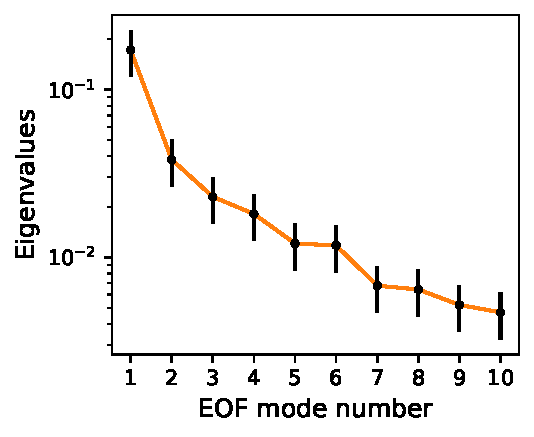
\includegraphics[scale=0.8]{texfiles/figs/EOF_north_test.pdf}
    \caption{The eigenvalues of the 10 first leading EOFs. The error bars correspond to the typical error of each EOF}
    \label{fig:eof_test}
\end{figure}


